\scanpage{27}
\figure{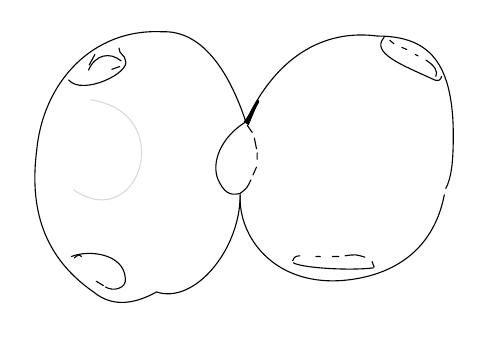
\begin{tikzpicture}[x=.009cm,y=-.009cm,line cap=round]
\draw (437,240) .. controls (407,150) and (365,111) .. (319,113)
 .. controls (220,108) and (151,185) .. (142,280)
 .. controls (130,373) and (159,436) .. (222,480)
 .. controls (251,504) and (284,495) .. (311,480)
 .. controls (364,498) and (429,421) .. (429,343);
\draw (437,240) .. controls (483,140) and (555,110) .. (622,119)
 .. controls (699,119) and (735,159) .. (729,286)
 .. controls (728,309) and (724,325) .. (719,334);
\draw (717,343) .. controls (701,425) and (640,459) .. (571,464)
 .. controls (475,470) and (426,401) .. (429,343);
\draw (437,240) .. controls (400,263) and (388,299) .. (398,322)
 .. controls (406,339) and (414,345) .. (429,341);
\draw (439,245)--(446,255) (449,263)--(452,278)
 (453,284)--(453,293) (452,304)--(447,315);
\draw (444,322) .. controls (439,333) .. (429,341);
\draw[line width=1.1pt] (454,211)--(438,240);
\fill (434,240)--(441,245)--(455,211)--cycle;
\draw (187,181) .. controls (207,204) and (276,170) .. (267,153)
 .. controls (267,146) and (258,145) .. (258,136);
\draw (215,167) .. controls (225,145) and (245,141) .. (261,154);
\draw (248,166)--(259,162) (216,160)--(224,145);
\draw (191,430) .. controls (216,420) and (265,426) .. (267,461)
 .. controls (269,475) and (250,480) .. (239,473);
\draw (195,432)..controls (201,427)..(205,430) (226,465)--(236,471);
\draw (632,121) .. controls (612,143) and (660,161) .. (699,179)
 .. controls (710,185) and (712,180) .. (713,176);
\draw (640,125)--(646,130) (657,135)--(664,138)
 (676,145)--(680,147);
\draw (691,153) .. controls (704,161) and (708,169) .. (705,176);
\draw (504,439) .. controls (519,447) and (589,450) .. (617,446);
\draw (503,436) .. controls (506,430) .. (513,429);
\draw (536,430)--(542,430) (559,430)--(568,430)
 (577,429) .. controls (592,427) .. (605,431) (615,437)--(618,445);
\draw[gray!30] (218,209) .. controls (342,227) and (287,400) .. (194,336);
\end{tikzpicture}}
\diagram{\begin{tikzcd}[column sep=large]
\left.\begin{array}{l}
4\text{ hexagones}\\16\text{ arêtes}\\10\text{ sommets}
\end{array}\right\}
\arrow[r,Rightarrow] &
\begin{array}{l}8\text{ hexagones}\\82\text{ arêtes}\\16\text{ sommets}\end{array}
\\
\begin{array}{l}(\text{dont }4\text{ ramifiés})\\\text{d'ordre}\end{array}&
\end{tikzcd}}
\begin{gather*}
\unsure{2|\deleted{6}\inserted{2}}\text{ hexag.}\\9\text{ arêtes}\\6\text{ sommets}
\end{gather*}
\figure{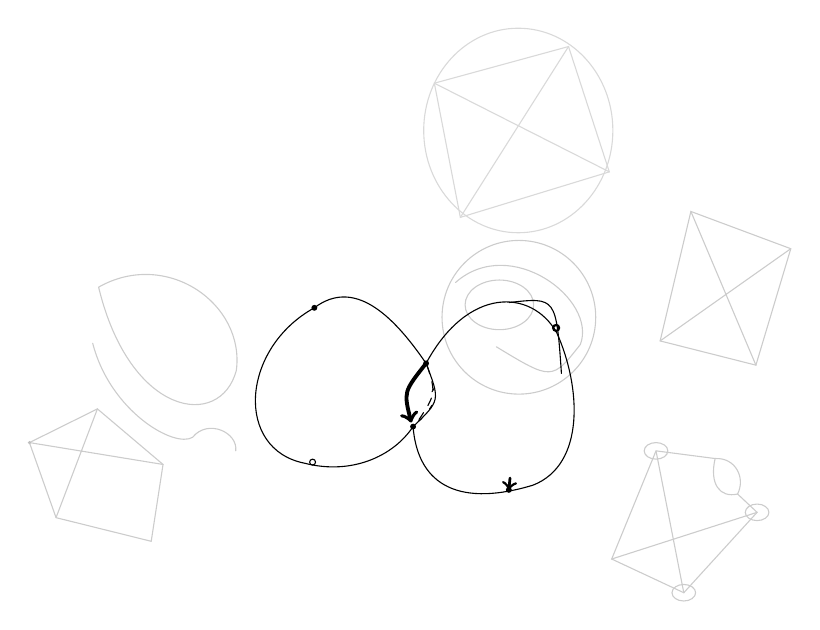
\begin{tikzpicture}[x=.0075cm,y=-.0075cm,line cap=round]
\draw[gray!30] (320,-440) ellipse (160 and 173);
\draw[gray!30] (178,-520)--(405,-582)--(474,-370)--(222,-293)--cycle;
\draw[gray!30] (178,-520)--(474,-370) (405,-582)--(222,-293);
\draw[gray!40] (-390,-175) .. controls (-275,-240) and (-142,-147) .. (-157,-34) .. controls (-184,67) and (-337,45) .. (-390,-175);
\draw[gray!40] (-400,-80) .. controls (-370,36) and (-261,98) .. (-231,79) .. controls (-205,47) and (-154,71) .. (-158,102);
\draw[gray!40] (-507,88)--(-392,31)--(-281,125)--(-301,255)--(-462,215)--cycle;
\draw[gray!40] (-507,88)--(-281,125) (-392,31)--(-462,215);
\fill[gray!50] (-507,88) circle (3);
\draw[gray!40] (321,-124) circle (130);
\draw[gray!40] (214,-183) .. controls (307,-265) and (454,-154) .. (425,-78) .. controls (377,-17) .. (283,-74);
\draw[gray!40] (288,-145) ellipse (58 and 42);
\draw[gray!40] (612,-303)--(781,-240)--(722,-43)--(560,-84)--cycle;
\draw[gray!40] (612,-303)--(722,-43) (781,-240)--(560,-84);
\draw[gray!40] (653,115) .. controls (687,113) and (705,147) .. (691,175) .. controls (661,182) and (643,158) .. (653,115);
\draw[gray!40] (553,102)--(653,115) (691,175)--(724,206)--(600,342)--(478,285)--(553,102);
\draw[gray!40] (553,102)--(600,342) (478,285)--(724,206);
\foreach \x/\y in {553/102,724/206,600/342}{\draw[gray!40] (\x,\y) ellipse (20 and 14);}
\draw (-25,-140) .. controls (-150,-71) and (-160,100) .. (-41,123) .. controls (37,143) and (108,112) .. (142,61);
\draw (-25,-140) .. controls (41,-190) and (106,-131) .. (164,-46);
\draw (164,-46) .. controls (234,-176) and (342,-173) .. (385,-98) .. controls (426,-7) and (434,125) .. (345,160) .. controls (209,201) and (149,151) .. (142,61);
\draw[->,line width=1.4pt] (164,-46) .. controls (126,2) .. (139,54);
\draw (164,-46) .. controls (188,17) .. (142,61);
\draw[dashed] (166,-42) .. controls (181,6) .. (146,58);
\draw (178,-4)--(174,2) (174,25)--(170,31) (156,48)--(151,52);
\draw (305,-149) .. controls (384,-158) .. (393,-29);
\foreach \x/\y in {-25/-140,164/-46,142/61,304/168}{\fill (\x,\y) circle (5);}
\draw[line width=.8pt] (384,-106) circle (5);
\draw (-28,121) circle (5);
\draw[->,line width=1pt] (306,148)--(304,168);
\end{tikzpicture}}% crop-candidate: scan 27
\diagram{\begin{tikzcd}[column sep=large]
\left.\begin{array}{l}
6\text{ sommets}\\(\text{dont }4\text{ ramifiés})\\
8\text{ arêtes}\\
4\ \deleted{\text{triangles}}\inserted{\text{carrés}}\;\text{--}
\end{array}\right\}
\arrow[r,Rightarrow]&
\begin{array}{l}
8\text{ sommets}\\\unsure{\text{d'ordre}|\text{dont}}4\\16\text{ arêtes}\\
8\ \deleted{\text{triangles}}\inserted{\text{carrés}}
\end{array}\arrow[d,bend right=20]\\
&\deleted{\unsure{1\times4|\text{dont }4|4\times4}\text{ d'ordre}}\ 4
\end{tikzcd}}
\figure{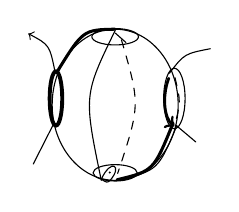
\begin{tikzpicture}[x=.8cm,y=.8cm,line cap=round]
\draw (0,0) ellipse (1 and 1.2);
\draw (0,1.08) ellipse (.37 and .13) (0,-1.08) ellipse (.35 and .13);
\draw[line width=1.4pt] (-.94,.1) ellipse (.1 and .43);
\draw (.94,.1) ellipse (.17 and .48);
\draw (.86,.5) .. controls (1.1,.81) .. (1.51,.89) (.96,-.32)--(1.28,-.59);
\draw[->] (-.95,.5)..controls (-1.04,.95)..(-1.38,1.13);
\draw (-.97,-.29)--(-1.3,-.94);
\draw (0,1.18)..controls (-.5,.15)..(-.22,-1.2);
\draw[dashed] (.1,1.03)..controls (.4,0)..(.04,-1.09);
\draw[line width=1.1pt] (-.93,.51)..controls (-.51,1.19)..(0,1.2) (.92,-.29)..controls (.61,-1.05)..(.03,-1.19);
\draw (0,1.14)--(.17,.99);
\draw (-.22,-1.18) .. controls (-.06,-.84) and (.12,-.97) .. (-.08,-1.2)
 .. controls (-.13,-1.24) .. (-.22,-1.18);
\fill (-.085,-1.075) circle (.018);
\draw[dashed] (.95,.43) .. controls (1.04,.05) .. (.95,-.31);
\draw[->,line width=1pt] (.85,.42) .. controls (.74,.12) and (.78,-.22) .. (.94,-.34);
\draw (.98,-.33) .. controls (.68,-1.04) .. (.04,-1.2);
\end{tikzpicture}}
\figure{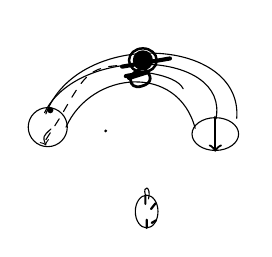
\begin{tikzpicture}[x=.8cm,y=.8cm,line cap=round]
\draw (-1.4,-.1) .. controls (-.89,1.26) and (1.73,1.13) .. (1.63,-.17);
\draw (-1.42,-.08) .. controls (-.89,1) and (1.52,.92) .. (1.3,-.18);
\draw (-1.08,-.31) .. controls (-.68,.59) and (.7,.71) .. (.97,-.33);
\draw (-1.37,-.31) circle (.31) (1.29,-.42) ellipse (.37 and .26);
\draw[->,line width=.8pt] (1.29,-.15)--(1.29,-.7);
\draw[dashed] (-1.4,-.51)--(-1.17,-.15)..controls (-.7,.67)..(.22,.68);
\fill (.14,.75) circle (.16);
\draw[line width=.9pt] (.14,.75) ellipse (.22 and .19);
\draw[line width=1pt] (.16,.62) .. controls (-.14,.58) and (-.1,.27) .. (.12,.34)
 .. controls (.31,.39) and (.28,.52) .. (.16,.62);
\draw (.24,.55) .. controls (.53,.5) and (.72,.42) .. (.78,.3);
\draw[->] (-1.32,-.34) .. controls (-1.45,-.46) .. (-1.4,-.6);
\draw[line width=1.5pt] (-.19,.65)--(.57,.78) (-.08,.47)--(.24,.57)--(-.13,.5);
\fill (-1.33,-.04) circle (.05);
\fill (-.45,-.37) circle (.025);
\draw (.2,-1.65) ellipse (.18 and .26);
\draw (.18,-1.39) .. controls (.13,-1.22) and (.28,-1.24) .. (.23,-1.45);
\draw[line width=.8pt] (.18,-1.4)--(.18,-1.53)
 (.34,-1.52)--(.27,-1.61) (.35,-1.79)--(.28,-1.83)
 (.2,-1.91)--(.2,-1.78);
\end{tikzpicture}}
\margin{Justine}% written upside down in the lower-left margin
\margin{26}
